\begin{figure}[h!]
  \centering
  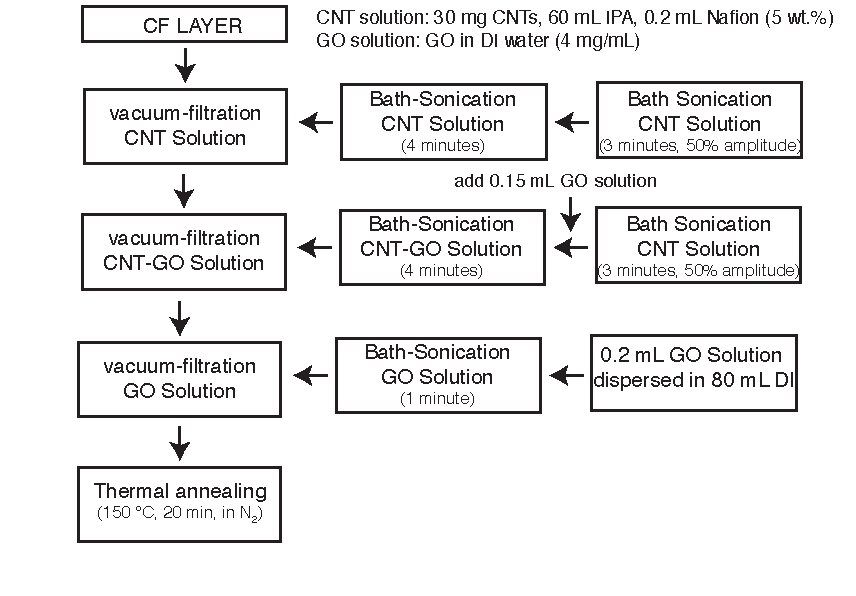
\includegraphics[width=5in]{paper5/FigS1.pdf}
  \caption{\textbf{FCM fabrication process.}}
  \label{figS1_AppD}
\end{figure}


\begin{figure}
  \centering
  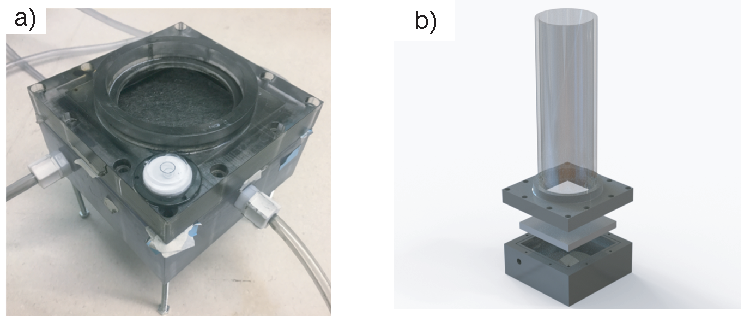
\includegraphics[width=6in]{paper5/FigS2.pdf}
  \caption{\textbf{Custom-made vacuum filtration device for FCM fabrication.} \textbf{(a)} Photo of the 3D-printed vacuum filtration device. \textbf{(b)} \textit{SolidWorks} representation of the 3D-printed vacuum filtration device.}
  \label{figS2_AppD}
\end{figure}

\begin{figure}
  \centering
  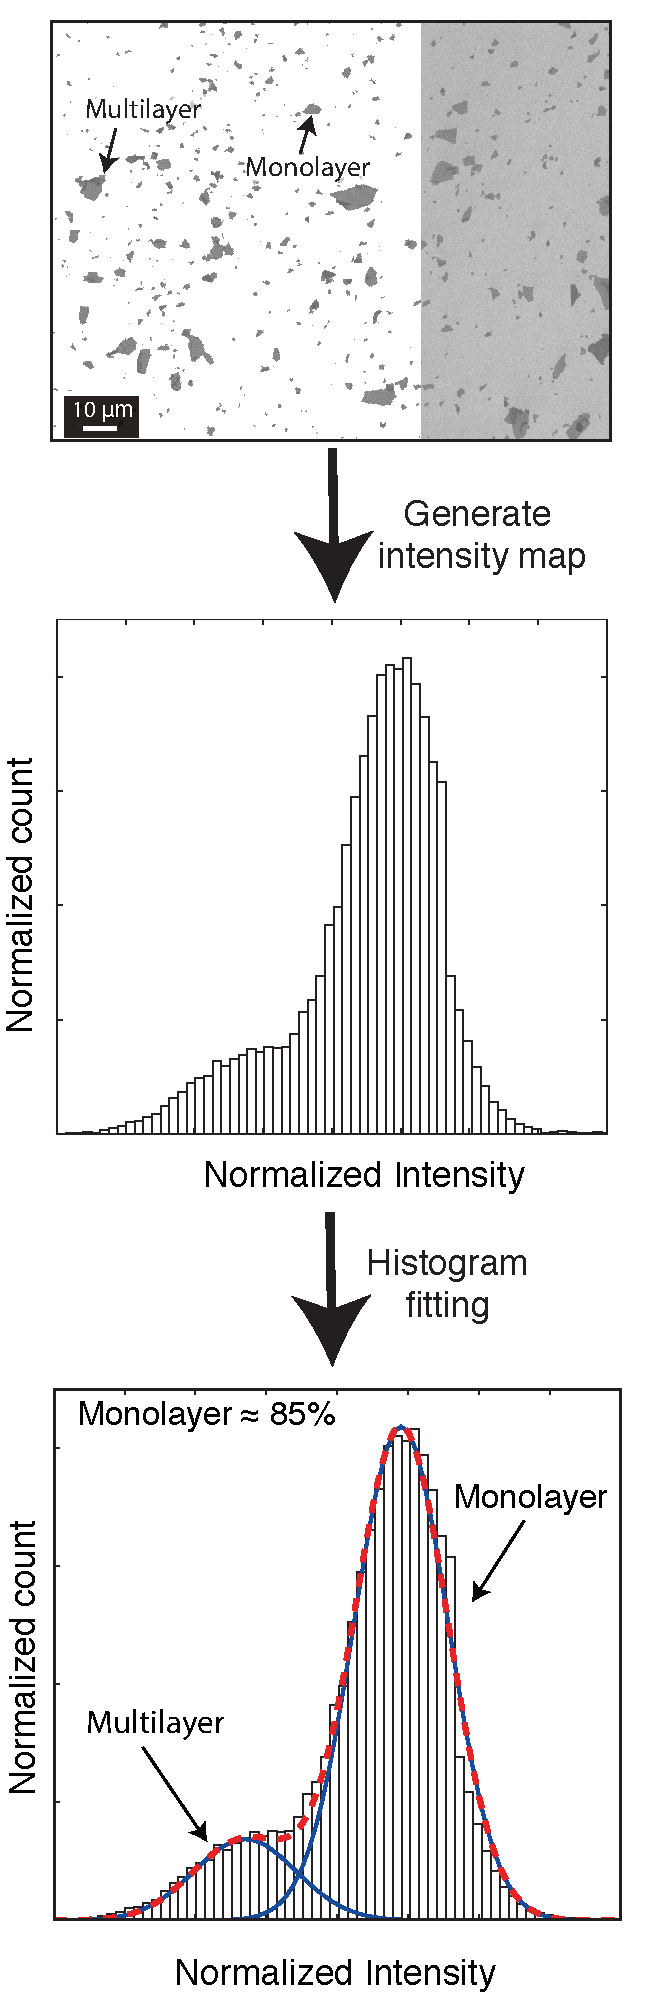
\includegraphics[width=5in]{paper5/FigS3.pdf}
  \caption{\textbf{Multi-cell cross-flow apparatus used for filtration tests.} (1) Membrane cell lines; (2) feed tank; (3) circulation pump; (4) control panel to adjust flow and pressure flow control valves; (5) flow-meter; (6) pH and conductivity sensor.}
  \label{figS3_AppD}
\end{figure}


\begin{figure}
  \centering
  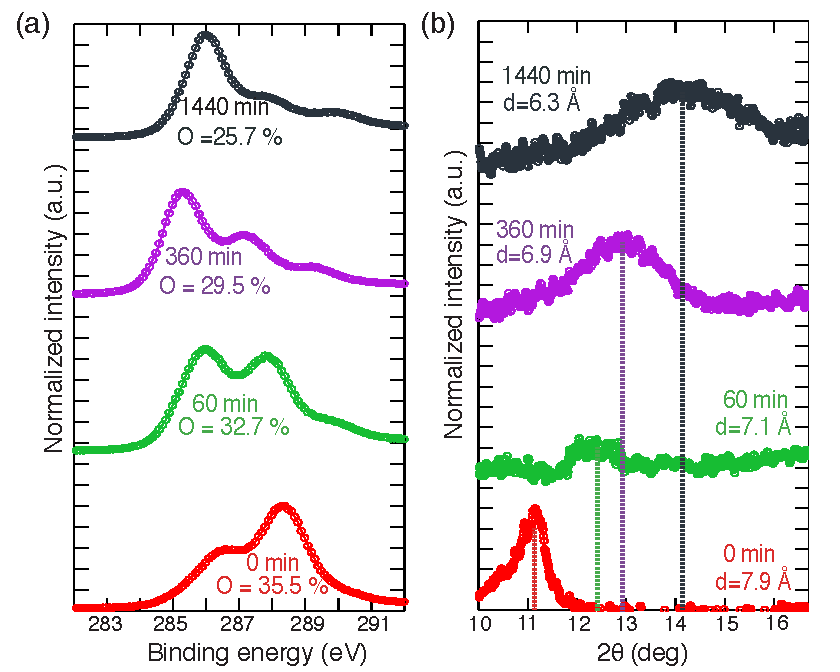
\includegraphics[width=6in]{paper5/FigS4.pdf}
  \caption{\textbf{SEM analysis of the hierarchical structure of FCM.} SEM surface images of \textbf{(a)} CF paper (1\textsuperscript{st} layer, substrate of the FCM), \textbf{(b)} intermediate CNT support layer (2\textsuperscript{nd} layer) and \textbf{(c)} GO selective layer (3\textsuperscript{rd} layer) at different magnifications.}
  \label{figS4_AppD}
\end{figure}

\begin{figure}
  \centering
  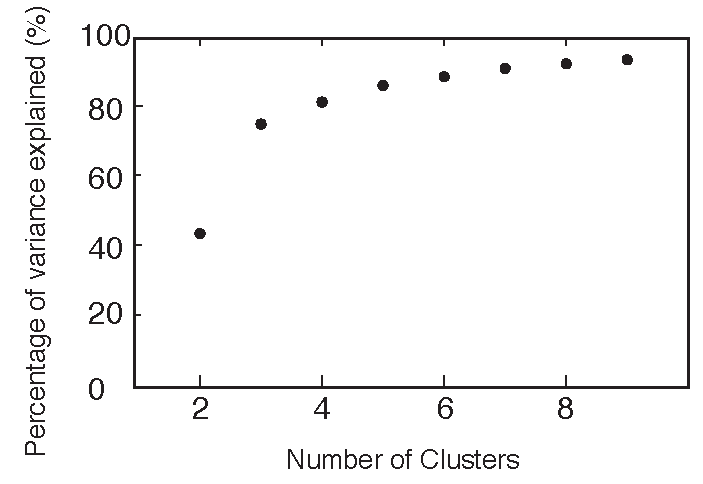
\includegraphics[width=6in]{paper5/FigS5.pdf}
  \caption{\textbf{Example of a mechanically-damaged FCM.} \textbf{(a)} CNT layer and \textbf{(b)} CF layer. \textit{ImageJ} software allows to recognized the superficial pores (in red) and calculate their areas.}
  \label{figS5_AppD}
\end{figure}



\begin{figure}
  \centering
  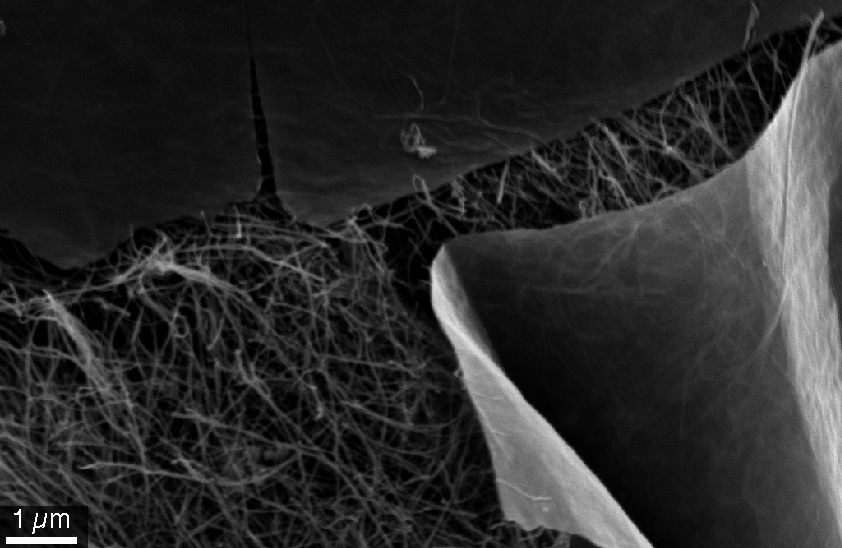
\includegraphics[width=3.5in]{paper5/FigS6.pdf}
  \caption{\textbf{Evaluation of the superficial mean pore size of the layers constituting the FCM.} The FCM has a crack that reveals the underneath CNT layer.}
  \label{figS6_AppD}
\end{figure}


\begin{figure}
  \centering
  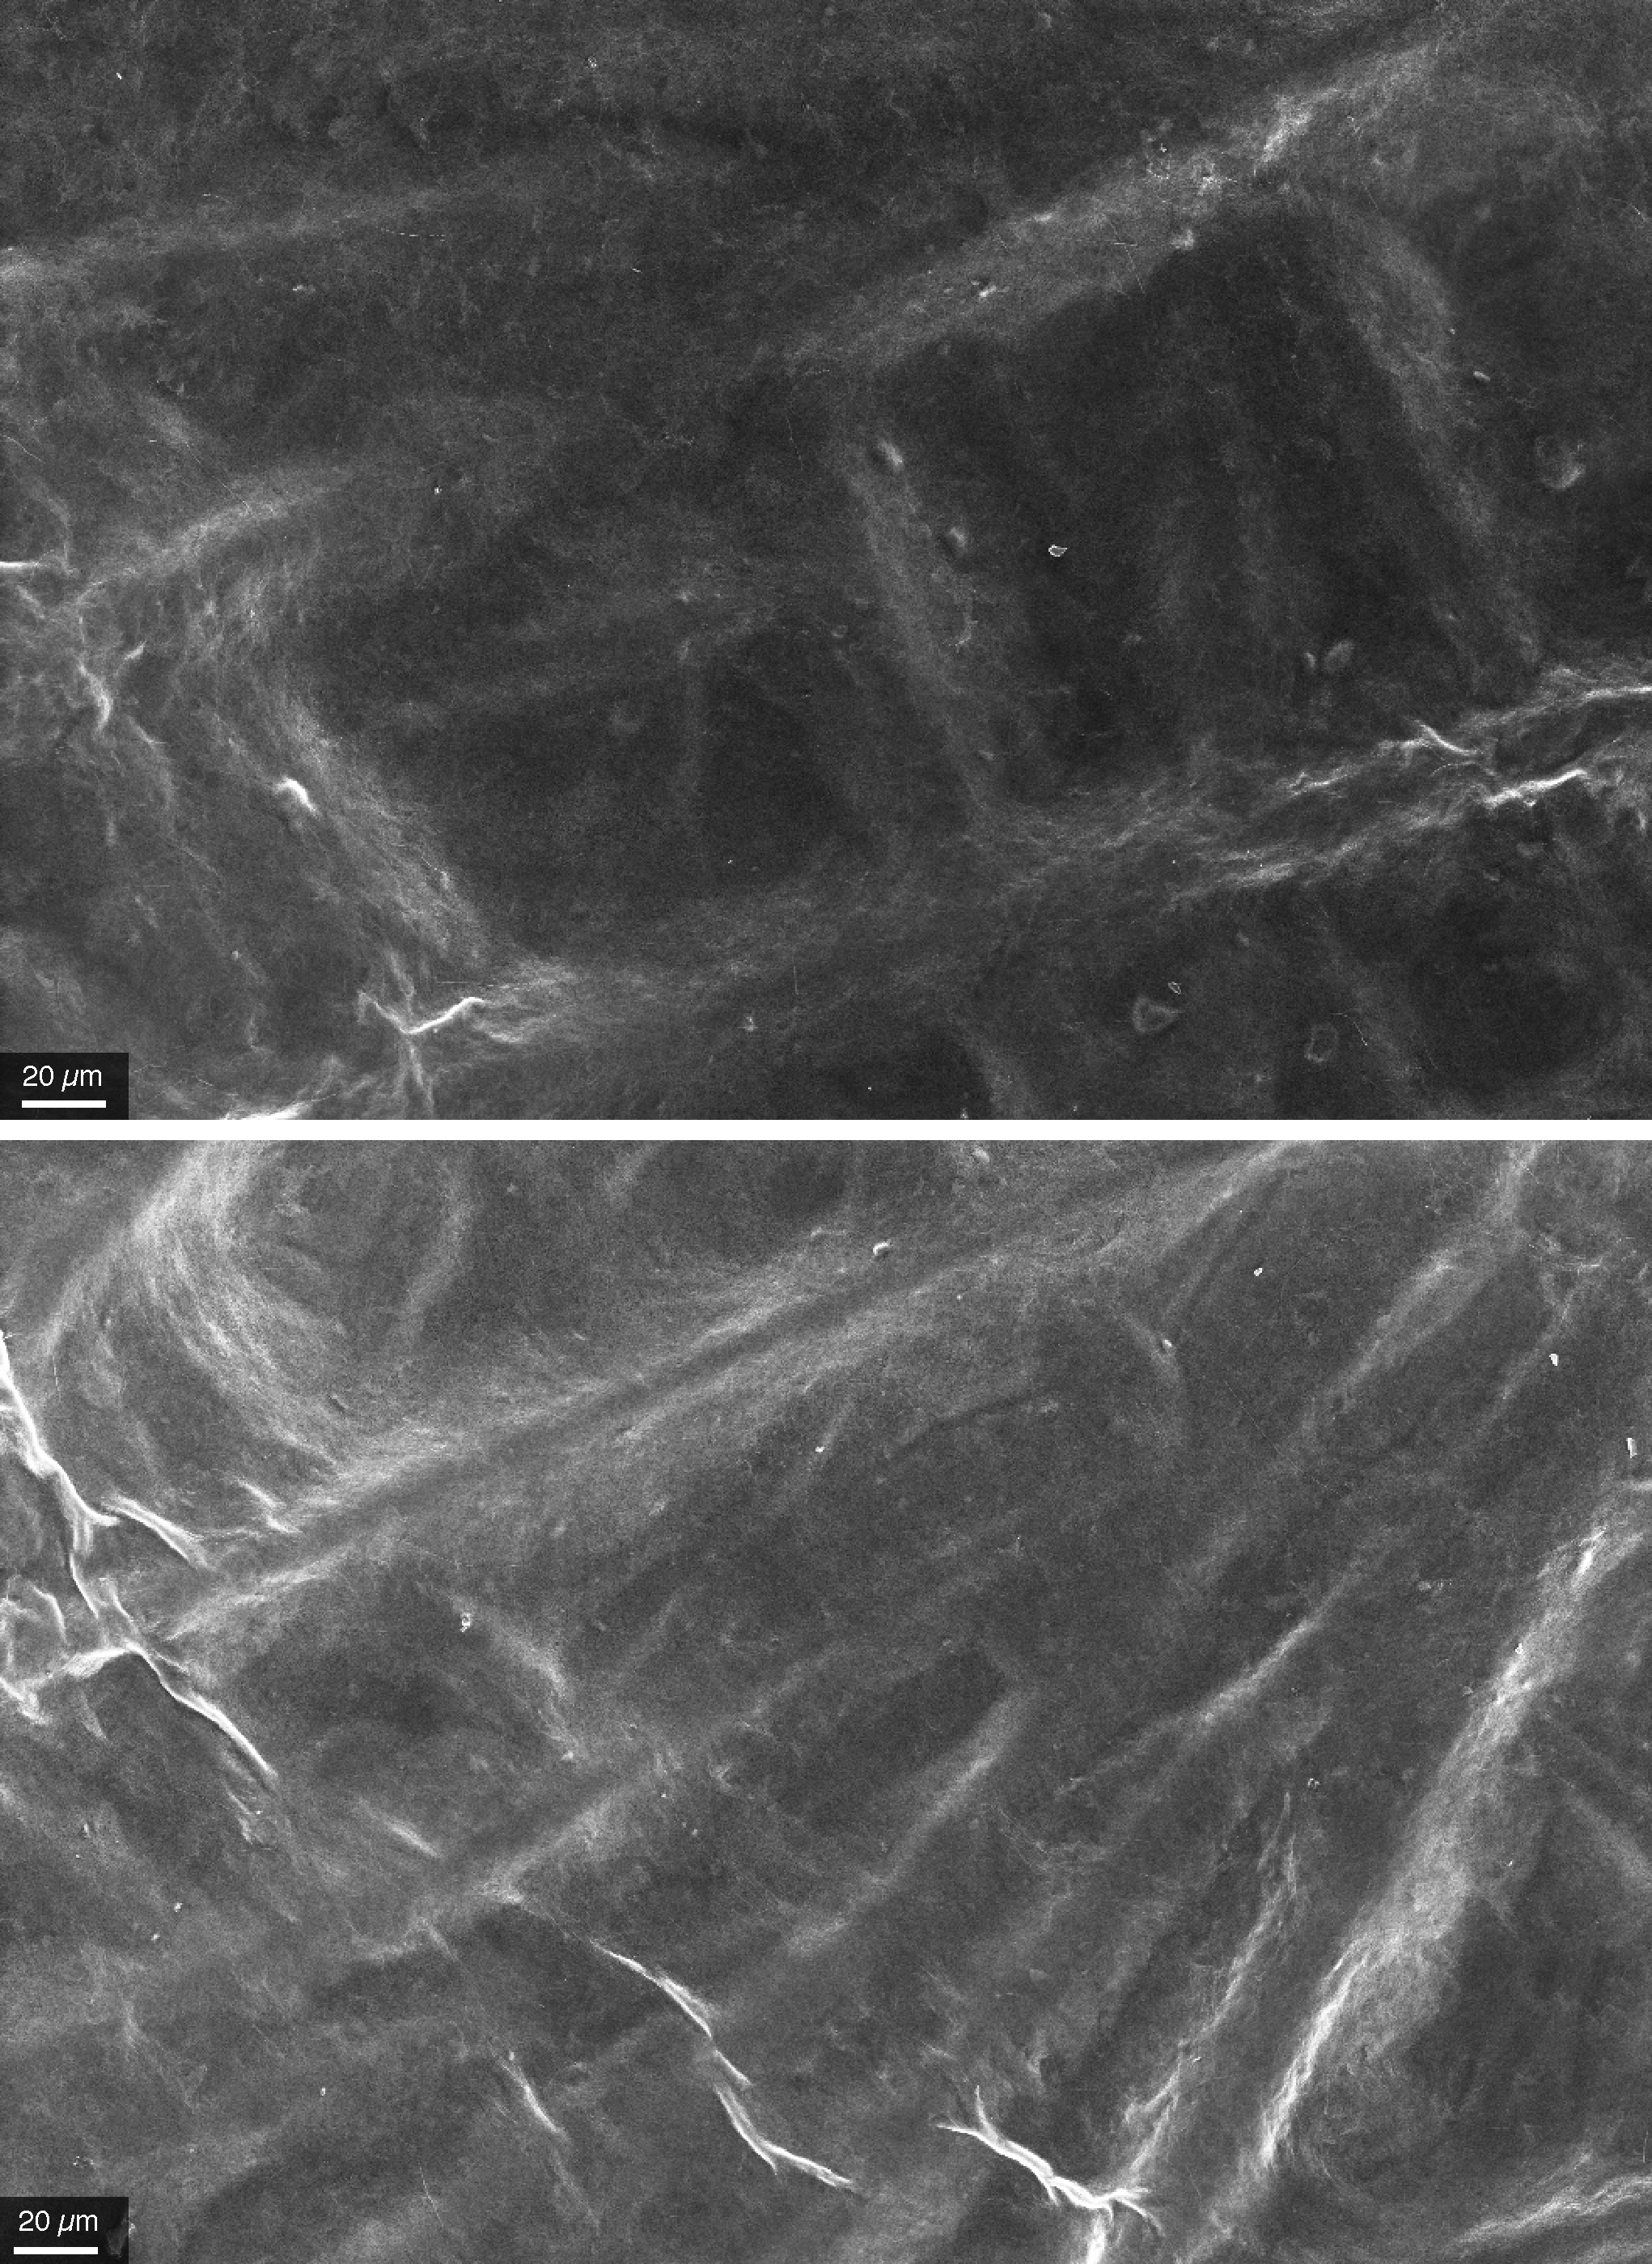
\includegraphics[width=3.5in]{paper5/FigS7.pdf}
  \caption{\textbf{FCM chemical stability to organic solvents.} FCM after being immersed in acetone (top) or water (bottom) reveals the same morphology.}
  \label{figS7_AppD}
\end{figure}


\begin{figure}
  \centering
  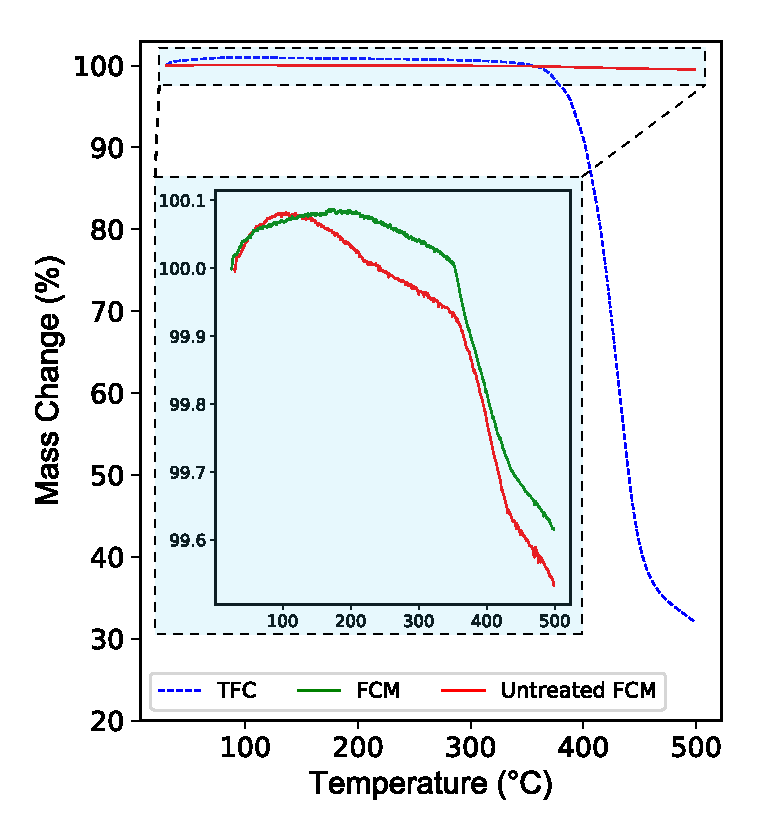
\includegraphics[width=5in]{paper5/FigS8.pdf}
  \caption{\textbf{Mass change over temperature of an untreated FCM (red line), a thermally treated FCM (green line) and a polyamide thin film composite (TFC) membrane (dashed blue line).} The untreated FCMs were not subjected to any annealing at 150 \textdegree C during the fabrication process whereas, the thermally treated FCMs were thermally reduced at 150 \textdegree C for 20 min during the fabrication process and then subjected to four sequential thermal annealing cycles of 15 min at 150 \textdegree C. TFC it was not treated before the annealing}
  \label{figS8_AppD}
\end{figure}

\begin{table}[h]
 \begin{center}
 \caption{\textbf{Decomposition of the C1s peak of the FCM after each thermal annealing cycle.}}
  \label{tblS1_AppD}
  \begin{tabular}{cccccc}
        \hline
        Functionality & Wavelength (eV) & 1\textsuperscript{st} & 2\textsuperscript{nd} & 3\textsuperscript{rd} & 4\textsuperscript{th}\\
        \hline
        C-C C=C & $\approx285$ & $64.5\pm1$ & $66.3\pm1$ & $65.0\pm1$ & $64.3\pm1$\\
        C-OH C-O-C & $\approx287$ & $14.1\pm1$ & $10.2\pm1$ & $15.0\pm1$ & $16.5\pm1$\\
        C=C-OH & $\approx289$ & $21.4\pm1$ & $23.5\pm1$ & $19.0\pm1$ & $20.2\pm1$\\
        \hline
  \end{tabular}
 \end{center}
 \small
\end{table}







